\documentclass[a4paper,11pt]{article}
\usepackage[utf8]{inputenc}
\usepackage[T1]{fontenc}
\usepackage[english]{babel}
\usepackage{lmodern}
\usepackage[margin=2.3cm]{geometry}
\usepackage{amsmath,amssymb}
\usepackage{booktabs}
\usepackage{graphicx}
\graphicspath{{../figures/}}
\usepackage[font=small,labelfont=bf,skip=4pt]{caption}
\usepackage{xcolor}
\usepackage{tikz}
\usetikzlibrary{positioning,calc,fit,backgrounds,arrows.meta}
\usepackage{pgfplots}
\pgfplotsset{compat=1.16}
\usepackage{enumitem}
\setlist{itemsep=2pt,topsep=3pt}
\usepackage{float}
\usepackage{microtype}
\usepackage{titlesec}
\titleformat{\section}{\normalfont\Large\bfseries}{\thesection}{0.6em}{}
\titleformat{\subsection}{\normalfont\large\bfseries}{\thesubsection}{0.6em}{}
\usepackage[colorlinks=true,linkcolor=blue!40!black,citecolor=blue!40!black,urlcolor=blue!50!black]{hyperref}

\definecolor{accentblue}{RGB}{37,99,235}
\definecolor{accentorange}{RGB}{217,119,6}
\definecolor{accentgreen}{RGB}{22,128,61}
\definecolor{accentgray}{RGB}{110,110,110}

\newcommand{\callout}[2]{\begin{center}\fcolorbox{#1}{#1!6}{\begin{minipage}{0.94\textwidth}\small #2\end{minipage}}\end{center}}

\title{\vspace{-1.2cm}\textbf{How Many Voices Does It Take to Clone One?}\\[4pt]
\large Data, results and research proposal: a scaling law for \textit{zero-shot}\\ voice cloning and an architecture that separates content and voice}
\author{Richard Viana\\[2pt]\small Project derived from the Machine Learning II final project --- IMPA Tech}
\date{\small Working document --- November 2026}

\begin{document}
\maketitle

\begin{abstract}
\noindent This document gathers everything the project has so far, so that an outsider can understand the work from it alone. We start from a speech synthesis system whose style is copied from a reference recording (Tacotron~2 + VAE) and use it as a cheap test bench for a data question: \emph{how many speakers, and how many sentences per speaker, does a model need to see in training to copy the voice of someone it has never heard?} In 33 controlled training runs (a grid of $N$ speakers $\times$ $K$ sentences, up to $N=200$), trained voices depend on $K$ and new voices depend on $N$. Measured on 38 never-heard voices, copying rises from 57\% to 70\% and 79\% with 8, 32 and 128 speakers, at no cost in intelligibility; with only three points and one seed, the shape of this curve (the exponent) is not yet identifiable. Five attempts to work around the shortage of speakers failed (reference swapping, a contrastive loss, a pretrained speaker vector, pseudo-speakers via speed change, averaging references), and the per-voice analysis indicates that the bottleneck is the \emph{decoder} being able to render the voice, not the encoder describing it. A critical review shows that part of the measured difficulty comes from the yardstick itself (copying is measured against the default voice) and proposes a ``coverage + attraction to the default voice'' model. Measuring directly on the generated audio how many bits about the voice pass through the system, the reference and the latent carry 4 to 5 bits about which of 38 voices is speaking, and the output only 0.3 (8 speakers) to 1 bit (128): the decoder is the bottleneck, and the gain from more speakers comes from it reaching more voices, not from becoming more precise on each one (about 0.3 bit per doubling). From this we propose (i) an information-theoretic description of zero-shot cloning and (ii) a two-stage architecture in which the voice is learned from \emph{untranscribed} audio, with falsifiable predictions to be tested on a dedicated GPU. The target application is dubbing into languages with few recorded speakers, such as Portuguese.
\end{abstract}

\tableofcontents
\newpage

%=====================================================================
\section{Motivation and question}

The long-term goal is \textbf{dubbing films}: given the translated text and the original actor's audio, generate speech in the target language with the actor's voice and style. This requires \emph{zero-shot} voice cloning: the model receives a short clip of a voice it has never heard and speaks new text with it.

Current cloning systems train on tens of thousands of hours and thousands of speakers. Languages such as Portuguese have transcribed corpora with a few dozen speakers. The question guiding the project is therefore one of data:

\callout{accentblue}{\textbf{Central question.} How many speakers ($N$) and how many sentences per speaker ($K$) does training need for the model to copy new voices without losing intelligibility? What is the functional form of this dependence, and what limits copying: the encoder describing the new voice, or the decoder being able to reproduce it?}

The model used (Tacotron~2 + VAE) is old and is not what one would use in a product today (Section~\ref{sec:limites}). It was chosen as a \emph{test bench}: it allows dozens of controlled training runs on a student budget. What we intend to carry forward is the question, the protocol and the theory, to be confirmed on a current architecture.

%=====================================================================
\section{What the project already has}

\begin{enumerate}
\item \textbf{A Portuguese speech synthesis system with copied style}, trained in stages (English $\rightarrow$ Portuguese $\rightarrow$ emotion) from NVIDIA's pretrained Tacotron~2. Word errors (WER, via Whisper): 2.2\% in English, 10.5\% in Portuguese; the pitch of the generated speech follows that of the reference (correlation 0.97 over 10 emotion references).
\item \textbf{A documented correction}: the previous version of the work had a central result (``interpretable spectral attention'') that came from a code bug (a \texttt{view} without transposing time and frequency). The bug was fixed and the result withdrawn.
\item \textbf{The coverage experiment} ($N \times K$): 33 training runs, automatic evaluation of intelligibility and voice copying, including an evaluation on 38 never-heard voices.
\item \textbf{A theory note} with a two-level scaling law, predictions registered \emph{before} each experiment, and the outcome of each one (hits and misses).
\item \textbf{Reproducible code} (training, evaluation, law fitting, per-voice analysis), per-sample results versioned in the repository, and a copy in the project's \textit{bucket}.
\end{enumerate}

%=====================================================================
\section{Current architecture}

\begin{figure}[H]
\centering
\resizebox{\textwidth}{!}{%
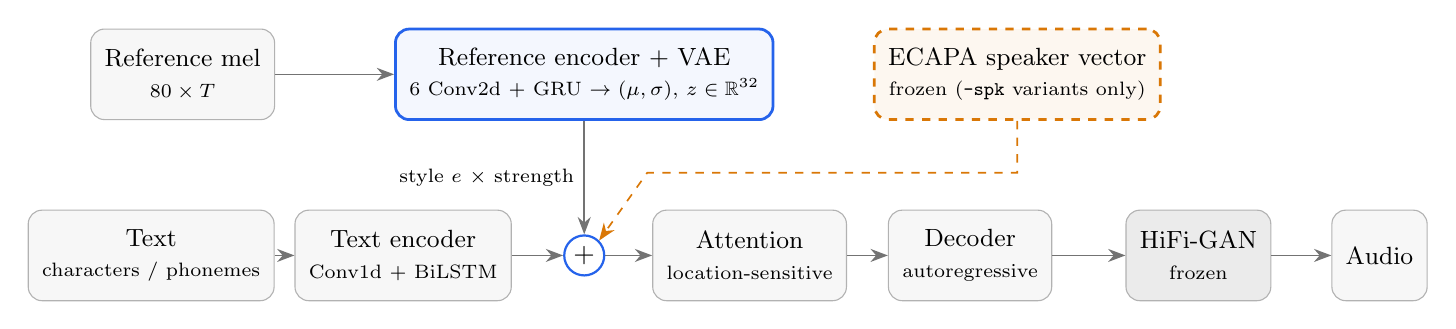
\begin{tikzpicture}[
  box/.style={rectangle, draw=black!30, rounded corners=5pt, fill=black!3, minimum height=1.15cm, align=center, font=\small, inner xsep=5pt},
  hl/.style={box, draw=accentblue, line width=1pt, fill=accentblue!5},
  op/.style={box, draw=accentorange, line width=1pt, fill=accentorange!6, dashed},
  frozen/.style={box, fill=black!8},
  arr/.style={-{Stealth[length=2.2mm]}, semithick, draw=black!55}
]
\node[box] (txt) at (0,0) {Text\\{\scriptsize characters / phonemes}};
\node[box] (enc) at (3.2,0) {Text encoder\\{\scriptsize Conv1d + BiLSTM}};
\node[circle, draw=accentblue, thick, fill=white, inner sep=1.5pt] (soma) at (5.5,0) {$+$};
\node[box] (att) at (7.6,0) {Attention\\{\scriptsize location-sensitive}};
\node[box] (dec) at (10.4,0) {Decoder\\{\scriptsize autoregressive}};
\node[frozen] (voc) at (13.3,0) {HiFi-GAN\\{\scriptsize frozen}};
\node[box] (wav) at (15.6,0) {Audio};
\node[box] (ref) at (0.4,2.3) {Reference mel\\{\scriptsize $80\times T$}};
\node[hl] (vae) at (5.5,2.3) {Reference encoder + VAE\\{\scriptsize 6 Conv2d + GRU $\rightarrow (\mu,\sigma)$, $z\in\mathbb{R}^{32}$}};
\node[op] (spk) at (11.0,2.3) {ECAPA speaker vector\\{\scriptsize frozen (\texttt{-spk} variants only)}};
\draw[arr] (txt) -- (enc); \draw[arr] (enc) -- (soma); \draw[arr] (soma) -- (att);
\draw[arr] (att) -- (dec); \draw[arr] (dec) -- (voc); \draw[arr] (voc) -- (wav);
\draw[arr] (ref) -- (vae);
\draw[arr] (vae.south) -- node[left, font=\scriptsize] {style $e$ $\times$ strength} (soma.north);
\draw[arr, dashed, draw=accentorange] (spk.south) |- (6.3,1.05) -- (soma.north east);
\end{tikzpicture}}
\caption{Tacotron~2 + VAE. The style vector $e$ (a projection of $z$), multiplied by a strength factor (1.0 = full style), is added to every position of the encoder memory. The dashed input (pretrained ECAPA speaker vector) exists only in the \texttt{-spk}/\texttt{-spkdrop} variants. 28.9\,M parameters.}
\label{fig:arq}
\end{figure}

\paragraph{Loss.} $\mathcal{L} = \mathcal{L}_{\text{mel}} + \mathcal{L}_{\text{gate}} + \beta\,\mathcal{L}_{\text{KL}} + \lambda\,\mathcal{L}_{\text{GA}}$: mel squared error, cross-entropy of the stop signal, VAE KL divergence with an increasing weight (about 0.024 at the end of coverage training) and guided attention ($\lambda = 2$, $\sigma=0.4$).

%=====================================================================
\section{Data and tools}

\begin{table}[H]
\centering\small
\begin{tabular}{@{}p{3.6cm}p{4.4cm}p{7.6cm}@{}}
\toprule
Dataset & Content & Use in the project\\
\midrule
LJSpeech & 1 female speaker, English, 23.7\,h & Default voice: 2,000 sentences in every coverage run\\
LibriTTS \textit{train-clean-100} & 247 speakers, English, $\approx$54\,h & The $N$ training speakers (up to 200 used)\\
LibriTTS \textit{test-clean} & 39 speakers, English & 38 external voices of the wide evaluation\\
TTS-Portuguese Corpus & 1 speaker, Portuguese, 3.8\,h & Portuguese system\\
VERBO & 12 speakers, 7 emotions, 1,167 utterances & Emotion stage\\
\midrule
Universal HiFi-GAN & pretrained vocoder & Mel $\rightarrow$ audio (frozen)\\
Whisper (\textit{faster-whisper}) & speech recognition & Intelligibility (WER)\\
Resemblyzer & speaker encoder & Voice-copying measure\\
ECAPA-TDNN & speaker encoder & \texttt{-spk} variants (model input)\\
\bottomrule
\end{tabular}
\caption{Data and auxiliary models. Copying is measured with an encoder (Resemblyzer) different from the one fed to the model (ECAPA), so as not to evaluate with the same yardstick used in training.}
\end{table}

\paragraph{Compute.} All coverage runs were trained on rented GPUs (Colab: L4 and A100), about 2.5\,h per 2,500-step run. No checkpoints of the coverage runs were kept, only the per-sample results and the latents of about 1,500 sentences per run.

%=====================================================================
\section{The coverage experiment}

\subsection{Design}

\begin{figure}[H]
\centering
\resizebox{0.95\textwidth}{!}{%
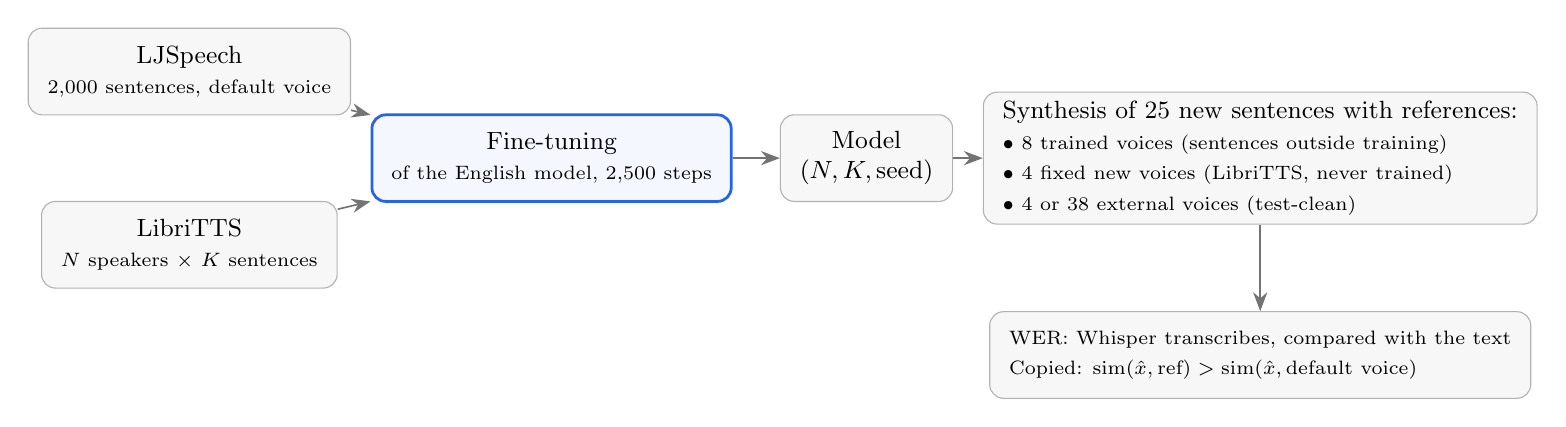
\begin{tikzpicture}[
  box/.style={rectangle, draw=black!30, rounded corners=5pt, fill=black!3, minimum height=1.1cm, align=center, font=\small, inner xsep=7pt},
  hl/.style={box, draw=accentblue, line width=1pt, fill=accentblue!5},
  arr/.style={-{Stealth[length=2.4mm]}, semithick, draw=black!55}
]
\node[box] (lj) at (0,1.1) {LJSpeech\\{\scriptsize 2,000 sentences, default voice}};
\node[box] (lt) at (0,-1.1) {LibriTTS\\{\scriptsize $N$ speakers $\times$ $K$ sentences}};
\node[hl] (tr) at (4.6,0) {Fine-tuning\\{\scriptsize of the English model, 2,500 steps}};
\node[box] (m) at (8.6,0) {Model\\$(N,K,\text{seed})$};
\node[box, align=left] (ev) at (13.6,0) {Synthesis of 25 new sentences with references:\\
{\scriptsize $\bullet$ 8 trained voices (sentences outside training)}\\
{\scriptsize $\bullet$ 4 fixed new voices (LibriTTS, never trained)}\\
{\scriptsize $\bullet$ 4 or 38 external voices (test-clean)}};
\node[box, align=left] (me) at (13.6,-2.5) {{\scriptsize WER: Whisper transcribes, compared with the text}\\{\scriptsize Copied: $\mathrm{sim}(\hat x, \text{ref}) > \mathrm{sim}(\hat x, \text{default voice})$}};
\draw[arr] (lj) -- (tr); \draw[arr] (lt) -- (tr); \draw[arr] (tr) -- (m); \draw[arr] (m) -- (ev); \draw[arr] (ev) -- (me);
\end{tikzpicture}}
\caption{Protocol. The selections are nested (the speakers of $N=8$ are contained in $N=32$, the sentences of $K=8$ in $K=32$), so that runs differ only in what was added.}
\end{figure}

\paragraph{Metrics.} \emph{WER}: word errors in the automatic transcription. \emph{Voice copied}: fraction of samples whose audio is closer (Resemblyzer cosine) to the reference than to the default voice. It is a binary measure, relative to the default voice, which has consequences (Section~\ref{sec:porvoz}). Variants also measure the similarity to the mean of up to 20 sentences of the reference speaker (\texttt{sim\_spk}).

\subsection{The $N \times K$ grid}

\begin{table}[H]
\centering\small
\begin{tabular}{@{}rrcccc@{}}
\toprule
$N$ & $K$ & WER trained & WER new & Copied: trained & Copied: new\\
\midrule
2 & 128 & 13\% / 11\% & 8\% / 5\% & 70\% / 74\% & 4\% / 2\%\\
8 & 8 & 21\% / 26\% & 14\% / 24\% & 45\% / 44\% & 26\% / 39\%\\
8 & 32 & 17\% & 14\% & 74\% & 47\%\\
8 & 128 & 11\% / 10\% & 8\% / 9\% & 91\% / 88\% & 51\% / 37\%\\
32 & 8 & 17\% / 17\% & 13\% / 9\% & 58\% / 51\% & 47\% / 47\%\\
32 & 32 & 13\% & 8\% & 80\% & 52\%\\
32 & 128 & 12\% / 10\% & 5\% / 5\% & 86\% / 86\% & 61\% / 57\%\\
128 & 8 & 12\% & 8\% & 52\% & 55\%\\
128 & 32 & 12\% / 13\% & 8\% / 8\% & 76\% / 66\% & 74\% / 56\%\\
200 & 32 & 12\% & 7\% & 66\% & 64\%\\
\bottomrule
\end{tabular}
\caption{Step 2,500, full style. ``New'' = the 4 fixed never-trained voices (25 sentences each). Two numbers = two seeds. The 4 voices give a noisy measure: the difference between seeds reaches 18 points.}
\label{tab:grade}
\end{table}

\begin{figure}[H]
\centering
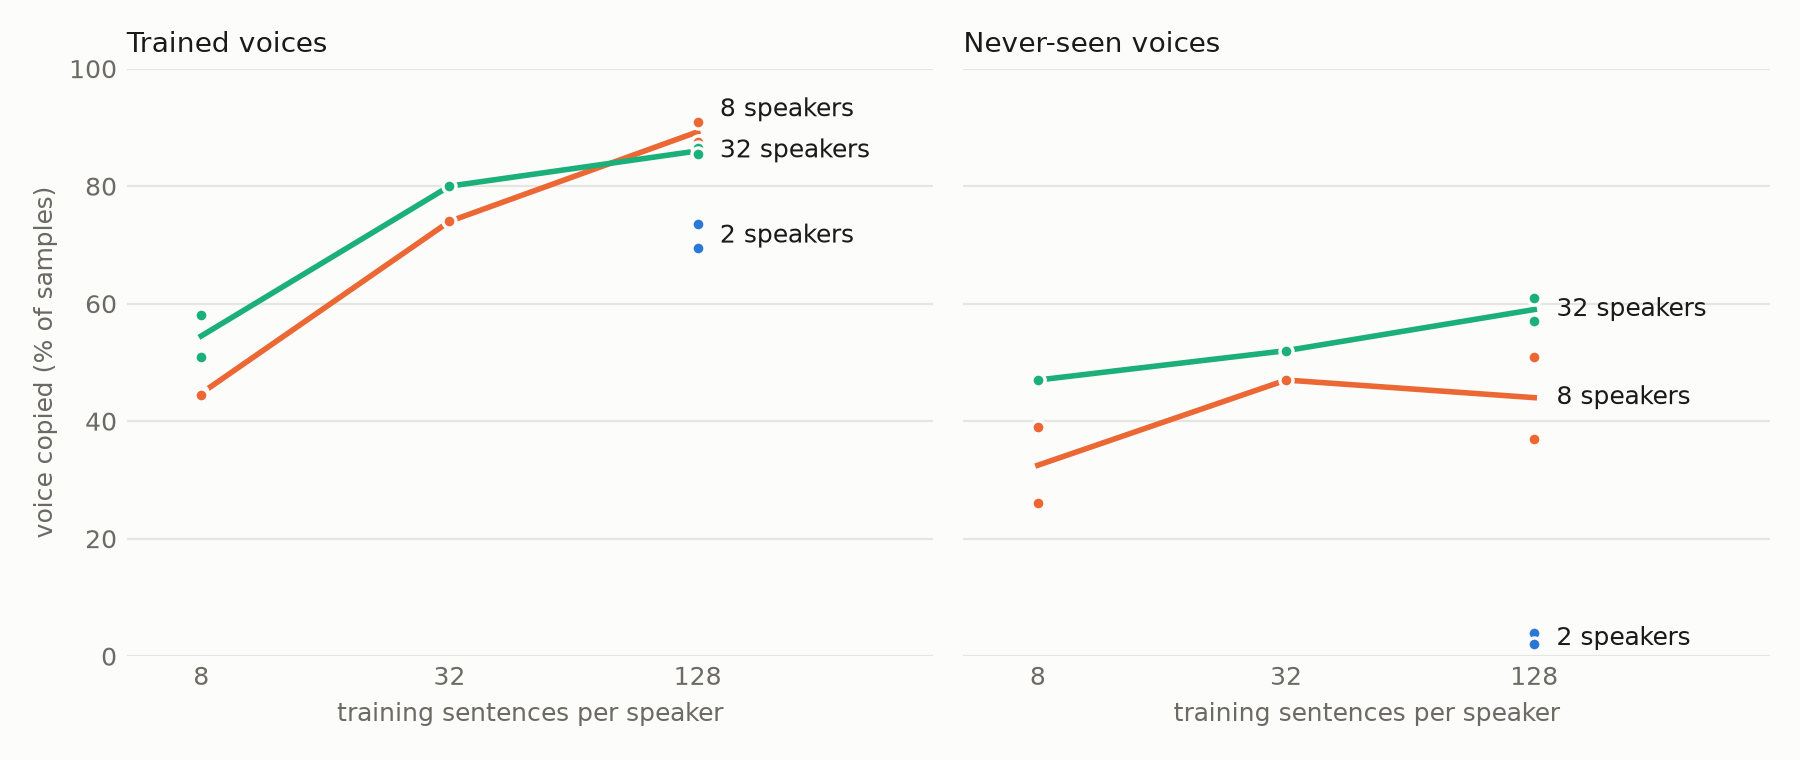
\includegraphics[width=0.82\textwidth]{fig_coverage}
\caption{Voice copied as a function of sentences per speaker ($K$) and number of speakers ($N$), original grid ($N\le32$).}
\end{figure}

\callout{accentgreen}{\textbf{Result 1 (two levels).} Trained voices depend on $K$: with 8 speakers, copying goes from 45\% ($K=8$) to 74\% (32) and 90\% (128). New voices depend on $N$: with $K=128$, from 3\% ($N=2$) to 44\% (8) and 59\% (32). Many speakers make up for few sentences: $32\times 8$ (256 sentences) copies new voices as well as $8 \times 128$ (1,024 sentences).}

\subsection{Wide evaluation: 38 never-heard voices}

Since 4 voices give a noisy measure, three runs with $K=32$ were evaluated on 38 speakers from LibriTTS \textit{test-clean} (950 samples per run). The 95\% intervals come from resampling the speakers (10,000 times), and the differences between runs are paired on the same speakers.

\begin{figure}[H]
\centering
\begin{minipage}{0.48\textwidth}
\centering
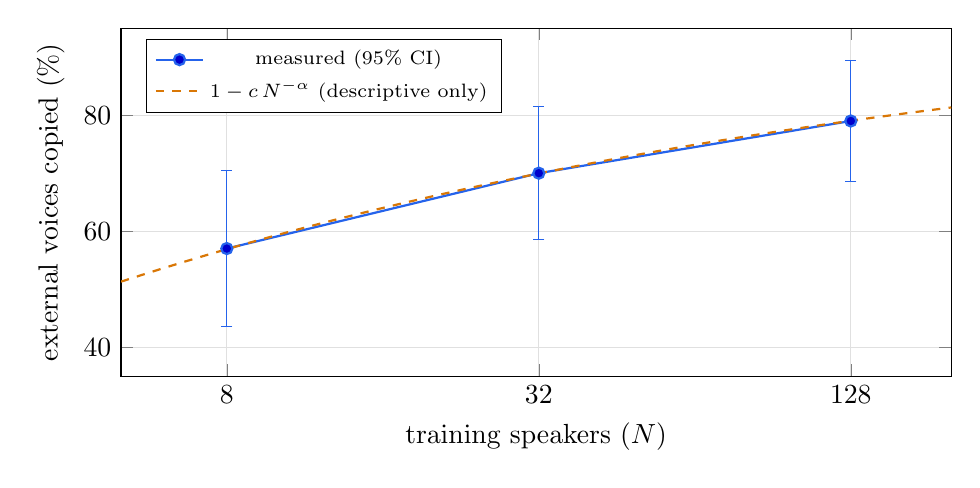
\begin{tikzpicture}
\begin{axis}[width=\linewidth, height=6cm, xmode=log, log basis x=2, xtick={8,32,128}, xticklabels={8,32,128},
  xlabel={training speakers ($N$)}, ylabel={external voices copied (\%)}, ymin=35, ymax=95, grid=major, grid style={black!12},
  xmin=5, xmax=200, legend style={font=\scriptsize, at={(0.03,0.97)}, anchor=north west}]
\addplot+[accentblue, mark=*, thick, error bars/.cd, y dir=both, y explicit] coordinates {(8,57) +- (0,13.5) (32,70) +- (0,11.5) (128,79) +- (0,10.5)};
\addlegendentry{measured (95\% CI)}
\addplot[accentorange, dashed, thick, domain=5:200, samples=40] {100*(1-0.74*x^(-0.26))};
\addlegendentry{$1-c\,N^{-\alpha}$ (descriptive only)}
\end{axis}
\end{tikzpicture}
\end{minipage}\hfill
\begin{minipage}{0.48\textwidth}
\small
\begin{tabular}{@{}lccc@{}}
\toprule
Run & Copied & WER & Per speaker\\
 & (95\% CI) & & $R=1 \rightarrow 4$\\
\midrule
$8\times32$ & 57\% (43--70) & 13\% & 66\% $\rightarrow$ 64\%\\
$32\times32$ & 70\% (58--81) & 12\% & 81\% $\rightarrow$ 79\%\\
$128\times32$ & 79\% (68--89) & 12\% & 88\% $\rightarrow$ 84\%\\
\bottomrule
\end{tabular}\\[6pt]
Paired gain: 13 points from 8 to 32 (CI 4--23); 9 points from 32 to 128 (CI 1.5--17).
\end{minipage}
\caption{Voice copying on 38 never-heard voices. The dashed curve is a power law passing through the three points ($\alpha=0.26$); with two parameters, three points and one seed, it describes and tests nothing: any $\alpha$ between about 0.06 and 0.53 would be compatible (Section~\ref{sec:revisao}). ``$R=4$'': style code taken from the mean of 4 sentences of the speaker.}
\label{fig:larga}
\end{figure}

\callout{accentgreen}{\textbf{Result 2 (more speakers keep paying off).} From 8 to 32 and from 32 to 128 speakers, copying of new voices rises by 13 and 9 points, with constant WER (12--13\%); the gain from 32 to 128 is real (the CI does not include zero). The earlier impression, from the 4 voices, that there was no gain above 128 speakers was measurement noise. What is \emph{not} established is the shape of the curve: the exponent and any extrapolation to thousands of speakers.}

\subsection{Attempts to work around the shortage of speakers (all negative)}

\begin{table}[H]
\centering\small
\begin{tabular}{@{}p{4.1cm}p{5.1cm}p{5.6cm}@{}}
\toprule
Idea & Hypothesis tested & Result\\
\midrule
Reference swap (\texttt{-swap}) and contrastive loss (\texttt{-contrast}) & The style code carries the sentence content & Nothing changes beyond the variation between seeds (e.g.\ $8\times128$: new 51\% $\rightarrow$ 38--39\%)\\
Frozen ECAPA speaker vector (\texttt{-spk}) & An encoder trained on thousands of voices describes new voices & The model ignores the input: without the VAE, 0\% copying\\
ECAPA + VAE \textit{dropout} (\texttt{-spkdrop}) & Force the voice to go through the vector & With 8 speakers the vector alone copies 71\% of the trained voices and 5\% of the new ones: it memorizes. With 32 speakers, vector + VAE = normal training\\
Pseudo-speakers via speed change (\texttt{-aug}) & Altered voices count as new speakers & Predicted 31\% (they do not count) or 50\% (they count); measured 28\%. Likewise with $K=128$: 42\% (predicted 44\% / 55\%). They do not count\\
Mean of 4 or 16 references & The error comes from the noise of a single reference & Helps on the 4 grid voices but not on the 38 external ones (drops 2 to 4 points); only reduces WER by 1 to 3 points\\
\bottomrule
\end{tabular}
\caption{Variants tested, with predictions registered beforehand in the cases indicated.}
\label{tab:neg}
\end{table}

\callout{accentorange}{\textbf{Result 3 (what does not solve it).} Neither a better encoder, nor better references, nor losses on the latent, nor simple artificial voices replace the decoder having heard many real voices.}

\subsection{Which voices fail, and why}
\label{sec:porvoz}

Rank correlations over the 38 external speakers (\texttt{scripts/coverage/voice\_hardness.py}):
\begin{itemize}
\item \textbf{The difficulty belongs to the voice:} the per-speaker copy rate correlates 0.75 between $N=8$ and 32, 0.74 between 32 and 128, 0.59 between 8 and 128. In every run there are voices at 0\% and at 100\%: copying is nearly all-or-nothing per voice.
\item \textbf{High-pitched voices fail more} ($-0.53$, $-0.52$, $-0.37$ between copying and the reference F0). The default voice is female; copying increases with the distance (in the latent) to the default voice (0.47; 0.58; 0.53). Part of the failure is attraction to the default voice, and part may be an artifact of the relative measure.
\item \textbf{The distance to the nearest trained voice predicts failure with few speakers and stops predicting it with many:} $-0.33$ ($N=8$), $-0.40$ ($N=32$), $+0.13$ ($N=128$).
\end{itemize}

\subsection{Information in the style latent}

\begin{table}[H]
\centering\small
\begin{tabular}{@{}lccc@{}}
\toprule
Run & Bits per sentence (KL) & Bits about the speaker (approx.) & $\log_2$(no.\ of speakers)\\
\midrule
$2\times128$ & 64 & 5 & 1.6\\
$8\times32$ & 67 & 10 & 3.2\\
$32\times32$ & 72 & 16 & 5.0\\
$128\times32$ & 73 & 19 & 6.9\\
$200\times32$ & 72 & 20 & 7.4\\
\bottomrule
\end{tabular}
\caption{The KL per sentence is an upper bound on the information that passes through the latent (all 32 dimensions are active in every run). ``Bits about the speaker'' uses a Gaussian approximation (total covariance over within-speaker covariance); the review (Section~\ref{sec:revisao}) shows that the bias is small, but that the number measures a continuous voice vector, not the identity among the $N$ speakers. About 80\% of the latent variance is between speakers, and the distance from the code to the default voice has a correlation of 0.83 with copying.}
\label{tab:info}
\end{table}

The style channel carries 65--73 bits per sentence (KL), but most of it pays for the narrow posterior; the estimated information about the voice stays near 17 bits and does not grow from $N=32$ to 200. The latent is not saturated: the limit is not capacity, it is how many voices the decoder has heard.

%=====================================================================
\section{Theory}

\subsection{Two-level law}

Speakers are drawn from a population; sentences are drawn within each speaker. In a finite-dimensional hierarchical (random-effects) model, the error on a trained voice has a term that falls with $K$, and the error on a new voice has a term that falls with $N$ and another with $NK$:
\begin{align*}
\text{trained not copied} &\approx a' + \frac{C}{K} + \frac{A'}{N}, &
\text{new not copied} &\approx a + \frac{A}{N} + \frac{B}{NK}.
\end{align*}
Fit on 16 runs: $a'=0.14$, $C=2.87$, $A'=0.22$ (RMSE 0.057); $a=0.39$, $A=1.08$, $B=10.3$ (RMSE 0.060). This is the form of the variance decomposition in two-stage sampling and of meta-learning bounds with Gaussian tasks.

\subsection{Two regimes and the exponent}

The form above predicts a $1/N$ decrease down to a floor $a\approx0.39$. The alternative $a + A/\sqrt N + C/\sqrt K$ fits equally well (RMSE 0.056, floor 0.19). The wide evaluation (Fig.~\ref{fig:larga}) shows not copied 43\% $\rightarrow$ 30\% $\rightarrow$ 21\%, which a power law $N^{-0.26}$ passes through exactly. By the criterion registered before the experiment, the ratio between the gains (0.7) favored the square-root law, but the statistical review (Section~\ref{sec:revisao}) shows that none of the laws can be distinguished from the others with these data.

\callout{accentblue}{\textbf{Proposed interpretation.} There are two regimes:
\begin{itemize}[leftmargin=12pt]
\item \emph{parametric}: the voice lives in a low-dimensional family of dimension $k$ that the decoder learns as a rule; the error falls as $k/N$ (fast);
\item \emph{non-parametric} (``coverage''): the decoder only reproduces voices close to the ones it has heard; the error is governed by the distance to the nearest trained voice, which falls as $N^{-1/d}$ in a voice space of intrinsic dimension $d$ (slow).
\end{itemize}
The dimension of the voice space measured in the latent is 7 to 10 (Section~\ref{sec:revisao}), which rules out the simplest version (failure proportional to the distance, which would require $d\approx4$ for $\alpha=0.26$); failure proportional to the squared distance requires $d\approx7.7$ and is compatible, without being a test. The per-voice analysis (distance to the nearest voice predicts failure at small $N$) and the failure of better encoders and references point to the coverage regime.}

\subsection{Consequences and predictions of the theory}
\begin{itemize}
\item If the regime is coverage, \textbf{improving the encoder does not change the exponent}; changing what the decoder has heard does (consistent with Table~\ref{tab:neg}).
\item An architecture that forces the voice dependence into a low-dimensional family should trade the slow decrease for a $1/N$ decrease, at the price of a floor if the real voice space has more dimensions than the module.
\item The extrapolations to thousands of speakers that appeared in the previous version of this document have been withdrawn: they have no statistical support.
\item The 32-dimensional latent is oversized for the voice: 8 to 10 dimensions should suffice for copying (prediction of the ``minimal model'').
\end{itemize}

\subsection{What already exists in the literature}
A survey (about 35 searches and 5 papers read in full) did not find an explicit law of voice copying as a function of $N$ and $K$. The qualitative fact ``thousands of speakers are needed'' appears as early as \cite{jia2018}, whose speaker-encoder table gives an apparent exponent of 0.21--0.25 (our calculation, with confounded factors). The analogue in speaker verification (few speakers vs.\ many sessions) is in \cite{tinyvox}. The forms $1/N + 1/(NK)$ and $1/\sqrt N + 1/\sqrt K$ come from meta-learning \cite{du2021,maurer2016}; exponents tied to the dimension of the data, from \cite{sharma2020,bahri2021}. The capacity of the style latent in bits has already been used in \cite{capacitron}. What appears to be new: the factorial $N\times K$ law for cloning, the link between the exponent and the dimension of the \emph{speaker} space (the samples are groups, not sentences), and the decomposition of the latent bits into voice and the rest. The search did not cover the ISCA Archive or IEEE Xplore.

%=====================================================================
\section{Critical review (three analyses without new training)}
\label{sec:revisao}

Three independent analyses, using only CPU on the saved data, reviewed the claims above (full reports in \texttt{reports/theory/}). What changed:

\paragraph{The yardstick.} With normalized speaker vectors, the measured margin has an exact form:
\[
m = \mathrm{sim}_{\text{ref}} - \mathrm{sim}_{\text{default}} = \left(\tfrac12 - \rho\right)\lVert e_{\text{ref}} - e_0\rVert^2,
\]
where $\rho$ is how much the output is pulled toward the default voice along the reference--default axis. The voice counts as copied if and only if $\rho<\tfrac12$, and the size of the margin is proportional to $\lVert e_{\text{ref}}-e_0\rVert^2$: voices similar to the default voice have tiny margins and switch sides due to noise. Pitch and similarity to the default voice explain 28--59\% of the voices' difficulty in the binary measure and only 2--9\% in the direct similarity to the reference. Part of the ``difficulty of high-pitched voices'' therefore belongs to the yardstick.

\paragraph{The exponent.} The power law $N^{-0.26}$ is exactly what two parameters do when passed through three points from one seed. In a simulation with the measured variance, this design recovers exponents between 0.06 and 0.53 when the true one is 0.26, and picks the correct law between 16\% and 62\% of the time. With measures that do not use the default voice, the apparent exponent rises to 0.41--0.55. On the 4-voice grid, the square-root law only wins because of the $N=2$ runs; without them, the four laws tested tie.

\paragraph{What holds.} Trained voices follow only $K$ (collapse in $K^{0.46}$, effect of $N$ equal to zero $\pm 0.07$). Copying is nearly all-or-nothing per voice (intraclass correlation 0.83--0.94; two thirds of the 38 voices fall below 10\% or above 90\%). The variation comes from the reference voice (standard deviation 0.095 in the margin) and not from the sentence (0.007); across seeds, the standard deviation of the copied fraction is 7.7 points, of which about 40\% is just resynthesis noise. The mean of 4 references does not improve copying on the 38 voices ($-2.5$ points, CI $[-6.4, +0.8]$) and reduces WER by 1.8 points.

\paragraph{Information and dimension.} Of the 64--75 bits per sentence of the KL, 62--70 pay for the narrow posterior; the Gaussian information about the sentence is 17--29 bits and the information about the voice about 17 bits in the mean $\mu$, stable from $N=32$ to 200. A cross-validated classifier recovers 5.1--5.3 of the 6.9 possible bits with 128 speakers. The voice occupies 6--8 useful directions (participation ratio 5.8--9.7) and the intrinsic dimension of the per-speaker means is 7--10 (TwoNN 9.7--10.6; Levina--Bickel 7.0--7.5).

\paragraph{A model that reproduces the facts.} A smoother that weights the trained voices by their number of sentences and competes with the default voice (2,000 sentences) gives the rule
\[
\text{copied} \iff K\textstyle\sum_i k(v,v_i) > M\,k(v,v_0),
\]
with $M$ the number of sentences of the default voice. With a voice spectrum $\lambda_j\propto 1/j$ (the latent measures an exponent of 1.05--1.1), this model reproduces the curve, the signs of the per-voice correlations, and the grid ($r=0.97$). These are five parameters chosen with three points, so this is not a test. The model also predicts that the speed-change pseudo-speakers should have counted, and they did not: this is the main open tension.

\paragraph{New, cheap predictions.}
\begin{itemize}
\item \textbf{Half the sentences of the default voice is equivalent to doubling $K$} for new voices (a direct consequence of the rule above). Costs two runs.
\item \textbf{An 8-dimensional latent} does not change copying; with 2 dimensions, it drops. The rate can go down to 25--30 bits per sentence without loss.
\item \textbf{$N=2{,}456$, $K=32$}: about 9\% of voices not copied under the coverage model versus 16\% or more under the laws with a floor; deciding this requires at least 200 evaluation voices.
\item \textbf{Without training}: the spectrum of the LibriTTS speaker vectors decides between the regimes and fixes the floor of a voice module of dimension $k$.
\item \textbf{Two stages}: copying follows $N_{\text{voice}}$ if the content units leak little voice information; a leak of weight 0.2 already imposes a floor of about 15\% of voices not copied.
\end{itemize}

%=====================================================================
\section{Information theory: where the voice bits are lost}
\label{sec:info}

Two theories were proposed by independent agents (coverage as source coding; copying as Bayesian hypothesis testing) and critiqued in three rounds. What remains is what survived both and can be measured without a model, from the audio itself (reports in \texttt{reports/theory/information/}).

\paragraph{The measure.} The voice information that passes through the system is $C = I(\hat Y; S)$: how much the voice of the generated audio $\hat Y$ says about which of the 38 external voices $S$ was the reference. It is estimated by identifying, with a speaker encoder, which reference each output came from; the confusion matrix gives lower bounds (Fano and cross-entropy). The ceiling is $\log_2 38 = 5.25$ bits.

\begin{figure}[H]
\centering
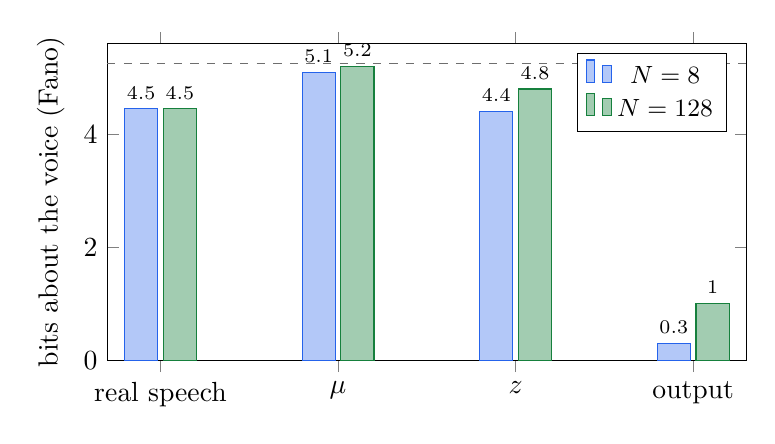
\begin{tikzpicture}
\begin{axis}[ybar, width=0.8\textwidth, height=5.6cm, bar width=12pt, ymin=0, ymax=5.6,
  symbolic x coords={real speech, $\mu$, $z$, output}, xtick=data, ylabel={bits about the voice (Fano)},
  legend style={font=\small, at={(0.97,0.97)}, anchor=north east}, nodes near coords, nodes near coords style={font=\scriptsize},
  every node near coord/.append style={/pgf/number format/fixed, /pgf/number format/precision=1}]
\addplot[fill=accentblue!35, draw=accentblue] coordinates {(real speech,4.45) ($\mu$,5.1) ($z$,4.4) (output,0.3)};
\addplot[fill=accentgreen!40, draw=accentgreen] coordinates {(real speech,4.45) ($\mu$,5.2) ($z$,4.8) (output,1.0)};
\draw[dashed, accentgray] (rel axis cs:0,0.9375) -- (rel axis cs:1,0.9375);
\legend{$N=8$, $N=128$}
\end{axis}
\end{tikzpicture}
\caption{Bit budget along the chain, on the same 38 voices (dashed line: ceiling of 5.25 bits). Real speech: verifier on the reference recordings (4.2--4.7). $\mu$ and $z$: Gaussian model in the latent. Output: measured on the generated audio. By the data processing inequality, information can only decrease along the chain; almost all of it is lost in the decoder.}
\label{fig:budget}
\end{figure}

\callout{accentgreen}{\textbf{Result 4 (the bottleneck is the decoder).} The reference and the latent carry 4 to 5 bits about which of the 38 voices is speaking; the generated audio carries 0.3 bit with 8 speakers and about 1 bit with 128 (Fano bound; by the cross-entropy bound, 0.75 and 2.0). The encoder is not the problem.}

\paragraph{Where the gain with $N$ comes from.} Writing $I(\hat Y;S) = H(\hat Y) - H(\hat Y\mid S)$, from $N=8$ to 128 the variety of reachable voices $H(\hat Y)$ rises by 1.44 bit (CI $[0.68, 2.32]$) and the per-voice noise $H(\hat Y\mid S)$ does not change ($+0.07$, CI $[-1.24, 1.54]$). The other theory, by an independent route (the width of the transition between copying and not copying, voice by voice), reaches the same conclusion: a decoder ``temperature'' of about 20, the same in all three runs. More speakers do not make the decoder more precise per voice; they increase the number of voice regions it reaches. It is coverage, not precision.

\paragraph{A law in bits.} The gain is 0.31 bit per doubling of $N$ (CI $[0.17, 0.47]$), measured at two points. If $C \approx c + 0.31\log_2 N$ continues to hold, the generated audio would carry 2.6 bits with 512 speakers and 3.2 with 2,048, and would only reach what real speech carries with about $10^5$ speakers (interval from $10^{3.6}$ to $10^{8.2}$). The law would be falsified by $C(2{,}048) < 2.25$ bits.

\paragraph{The negative results in one calculation.} The ECAPA vector alone transmits 0.00 bit (the decoder ignores it); with \textit{dropout}, 0.6--1.3. The mean of 4 or 16 references changes $C$ by between $-0.40$ and $+0.31$ bit, with no consistent direction. Style at 60\% lowers $C$ in 8 of 10 runs. Across 12 runs, the not-copied fraction and $C$ have a rank correlation of $-0.49$. Nothing that acts only before the decoder changes the bits that come out.

\paragraph{A priori prediction confirmed.} If each voice is decided by a likelihood ratio, longer reference sentences (more evidence) should make copying more all-or-nothing. Confirmed in all three runs: $+0.035$ (CI $[0.015, 0.053]$), $p=0.0002$ by permutation.

\paragraph{What died in the rounds of critique.} An optimal parameter-free Bayesian decoder (it predicts nearly every voice copied: it uses 22 times more evidence than the real one); the trained voice as a noisy point (it gets the effect of $K$ wrong); ``information per voice'' as a predictor of which voices fail; a stable exponent between 8 and 2,456 speakers; the hypothesis that per-voice capacity grows with $N$. Attraction to the default voice survives with an effective mass compatible with the 2,000 real sentences (2,300 to 5,000), but the predicted effect of halving them (4 to 9 points) requires about 6 runs per condition to be measured.

\callout{accentblue}{\textbf{Consequence for the architecture.} The target is neither a better encoder nor better references: it is to increase $H(\hat Y)$, the set of voices the decoder can produce. There are two levers: (i) give the decoder more voices, which the voice stage of Fig.~\ref{fig:proposta} does with untranscribed audio; (ii) a conditioning that lets the decoder interpolate between voices instead of falling into the nearest trained region (in the current model the style is added only once to the encoder memory; conditioning at every layer is the hypothesis to test). Every new run should measure $C$, $H(\hat Y)$ and $H(\hat Y\mid S)$ on 60 to 100 voices, and keep the generated audio for every point.}

%=====================================================================
\section{Limits of what we have}
\label{sec:limites}
\begin{itemize}
\item \textbf{Old architecture.} Tacotron~2 (2017) has been surpassed by language models over codec tokens and by \textit{flow matching}/diffusion models trained on tens of thousands of hours. Tacotron's attention is fragile and its quality hits a ceiling. The result only matters for the field if it repeats on a current model.
\item \textbf{Small scale.} $N\le200$, one seed in most cells, 2,500 steps. Three points in the wide evaluation do not distinguish a power law from a logarithm.
\item \textbf{One measure.} Copying depends on a speaker encoder and is relative to the default voice, which distorts the difficulty of voices similar to it (Section~\ref{sec:revisao}); there is no listening test and no naturalness measure.
\item \textbf{No checkpoints.} The bits-per-decoder-parameter calculation cannot be done with what was saved.
\end{itemize}

%=====================================================================
\section{Proposal}

\subsection{Question and hypothesis}

\callout{accentblue}{\textbf{Question.} Does copying of new voices depend on the number of speakers in the \emph{transcribed} audio, or on the number of speakers the voice module has heard, transcribed or not?\\[3pt]
\textbf{Hypothesis.} If the voice is learned by a separate stage, from untranscribed audio, copying comes to follow the number of speakers of that stage, with the same law; few transcribed speakers suffice for the content. To clone well, collect voices, not transcripts.}

\subsection{Proposed architecture: content and voice separated}

\begin{figure}[H]
\centering
\resizebox{\textwidth}{!}{%
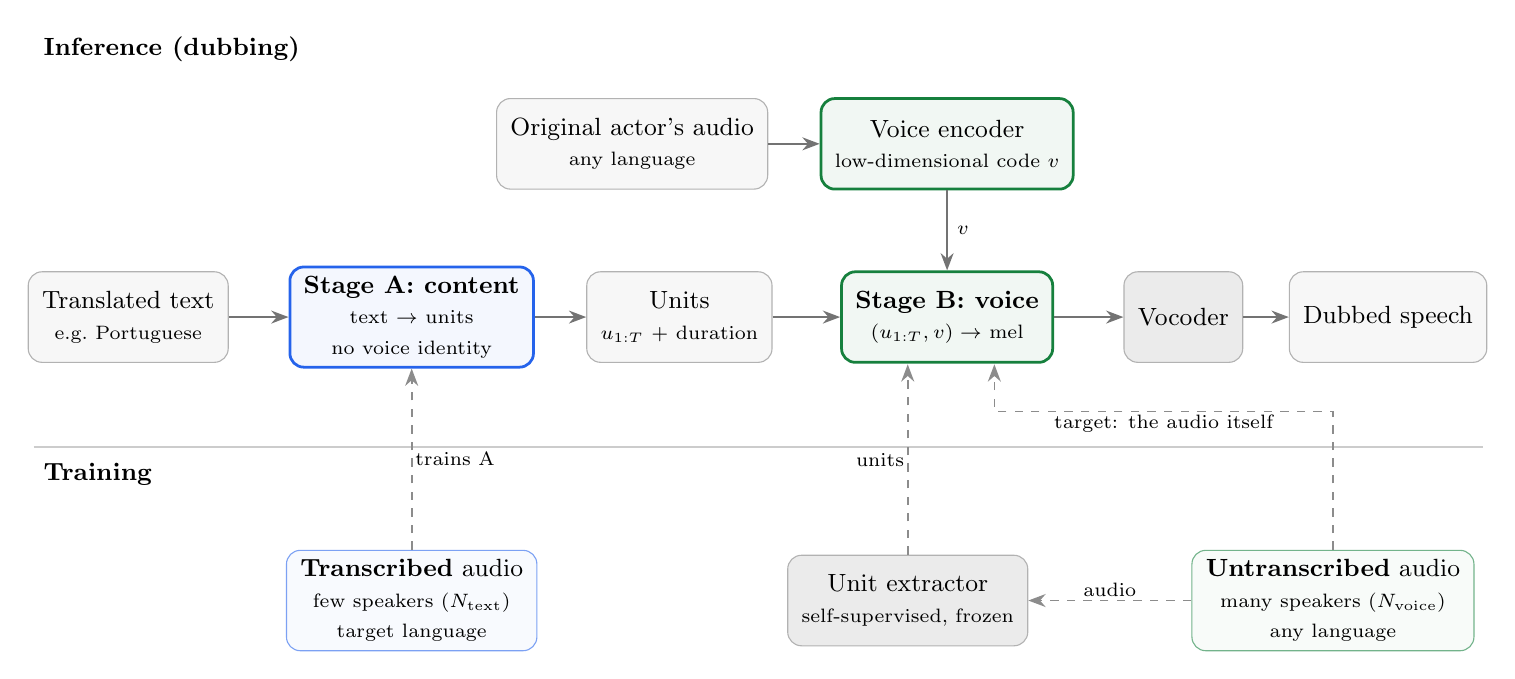
\begin{tikzpicture}[
  box/.style={rectangle, draw=black!30, rounded corners=5pt, fill=black!3, minimum height=1.15cm, align=center, font=\small, inner xsep=5pt},
  ca/.style={box, draw=accentblue, line width=1pt, fill=accentblue!5},
  cb/.style={box, draw=accentgreen, line width=1pt, fill=accentgreen!6},
  fz/.style={box, fill=black!8},
  arr/.style={-{Stealth[length=2.2mm]}, semithick, draw=black!55},
  tr/.style={-{Stealth[length=2.2mm]}, semithick, dashed, draw=black!45},
  lab/.style={font=\scriptsize, fill=white, inner sep=1pt}
]
\node[font=\small\bfseries, anchor=west] at (-1.2,3.4) {Inference (dubbing)};
\node[box] (txt) at (0,0) {Translated text\\{\scriptsize e.g.\ Portuguese}};
\node[ca] (A) at (3.6,0) {\textbf{Stage A: content}\\{\scriptsize text $\rightarrow$ units}\\{\scriptsize no voice identity}};
\node[box] (u) at (7.0,0) {Units\\{\scriptsize $u_{1:T}$ + duration}};
\node[cb] (B) at (10.4,0) {\textbf{Stage B: voice}\\{\scriptsize $(u_{1:T}, v) \rightarrow$ mel}};
\node[fz] (voc) at (13.4,0) {Vocoder};
\node[box] (out) at (16.0,0) {Dubbed speech};
\node[box] (ator) at (6.4,2.2) {Original actor's audio\\{\scriptsize any language}};
\node[cb] (ve) at (10.4,2.2) {Voice encoder\\{\scriptsize low-dimensional code $v$}};
\draw[arr] (txt) -- (A); \draw[arr] (A) -- (u); \draw[arr] (u) -- (B); \draw[arr] (B) -- (voc); \draw[arr] (voc) -- (out);
\draw[arr] (ator) -- (ve); \draw[arr] (ve) -- node[right, font=\scriptsize]{$v$} (B);
\draw[black!20] (-1.2,-1.65) -- (17.2,-1.65);
\node[font=\small\bfseries, anchor=west] at (-1.2,-2.0) {Training};
\node[box, fill=accentblue!3, draw=accentblue!60] (dA) at (3.6,-3.6) {\textbf{Transcribed} audio\\{\scriptsize few speakers ($N_{\text{text}}$)}\\{\scriptsize target language}};
\node[fz] (ssl) at (9.9,-3.6) {Unit extractor\\{\scriptsize self-supervised, frozen}};
\node[box, fill=accentgreen!3, draw=accentgreen!60] (dB) at (15.3,-3.6) {\textbf{Untranscribed} audio\\{\scriptsize many speakers ($N_{\text{voice}}$)}\\{\scriptsize any language}};
\draw[tr] (dA.north) -- node[lab, right]{trains A} (A.south);
\draw[tr] (dB.west) -- node[lab, above]{audio} (ssl.east);
\draw[tr] (ssl.north) -- node[lab, left]{units} (9.9,-0.6);
\draw[tr] (dB.north) -- (15.3,-1.2) -- node[lab, below]{target: the audio itself} (11.0,-1.2) -- (11.0,-0.6);
\end{tikzpicture}}
\caption{Proposal. Stage A learns what to say and needs text; stage B learns to render voices and is trained by reconstruction (units extracted from the audio itself $\rightarrow$ the same audio), without text. The targets of stage A are the units extracted from the transcribed audio. Dashed arrows are training; solid ones, inference. The scaling law predicts that copying of new voices follows $N_{\text{voice}}$, not $N_{\text{text}}$.}
\label{fig:proposta}
\end{figure}

Splitting into stages is not new in itself: there are systems that first generate content tokens and then the audio, and works that use untranscribed speech to reduce the need for text. What this proposal adds is \textbf{measuring which dataset voice copying comes from, and with what law}, with the exponent predicted beforehand, and the case of \textbf{different languages in the two stages}. Before investing, a dedicated search is needed to confirm that this has not been done.

\subsection{Planned experiments (dedicated GPU, NVIDIA RTX A4500, 20\,GB)}

\begin{table}[H]
\centering\small
\begin{tabular}{@{}p{0.6cm}p{4.6cm}p{5.4cm}p{4.2cm}@{}}
\toprule
& Experiment & Registered prediction & What it decides\\
\midrule
E0 & No training: spectrum of the LibriTTS speaker vectors; small listening test on the high-pitched voices & Spectrum in $1/j$ (coverage); listeners do not confirm the ``difficulty'' of the high-pitched voices & Regime; how much of the curve belongs to the yardstick\\
E0b & Half the sentences of the default voice ($M=1{,}000$) versus twice $K$ & Same effect on new voices & The coverage + attraction model\\
E1 & Repeat the $N$ sweep (8 to 2,456, full LibriTTS) on an open current architecture, in a small configuration; $N\in\{8,32,128,512,2048\}$, 3--5 seeds, 60--100 evaluation voices $\times$ 10 sentences, continuous metric without a default voice & Gain continues up to 2,048; not copied $\approx$9\% (coverage) or $\ge$16\% (floor) & Whether the law belongs to Tacotron or to the task, and which law\\
E2 & Two-stage architecture: $N_{\text{text}}=8$ fixed, $N_{\text{voice}}$ from 8 to 2,456 & $C$ follows $N_{\text{voice}}$ (about 0.3 bit per doubling); WER follows $N_{\text{text}}$; voice leakage in the units below about 0.2 bit per sentence & The central hypothesis\\
E3 & Stage B in English, stage A in Portuguese with few speakers & Copying of new voices close to that of E2; Portuguese WER close to the current system (10\%) & Dubbing with little data\\
E5 & Same decoder with style conditioning every layer (adaptive normalization) versus style added to the encoder memory, $N \in \{8, 128\}$ & Larger $H(\hat Y)$ and $C$ with conditioning at every layer, same per-voice noise & Whether the bottleneck is the conditioning mechanism\\
E4 & Smaller voice latent (32 $\rightarrow$ 16, 8, 4, 2) and larger KL & Copying unchanged with 8 dimensions and a rate of 25--30 bits; drops with 2 & The ``minimal model''\\
\bottomrule
\end{tabular}
\caption{Plan. Each prediction is written into the theory note before running. The evaluation design comes from a power simulation with the measured variance: from about 40 voices on, the bottleneck is the number of seeds. Checkpoints will now be kept for the information-per-parameter analysis.}
\end{table}

\paragraph{Success criterion.} The thesis holds if, in E2, copying of new voices with 8 transcribed speakers and thousands of untranscribed speakers falls within the interval of a model trained with thousands of transcribed speakers. If E1 does not reproduce the law on a current architecture, the work reduces to a study of Tacotron, and the architecture proposal must be revised before E2.

\subsection{Expected outputs}
\begin{enumerate}
\item \textbf{Workshop paper} with what already exists: ``How Many Voices Does It Take to Clone One? A Scaling Law for Zero-Shot Voice Cloning'' (controlled study, two-level law, negatives, per-voice analysis).
\item \textbf{Main paper}, if E1--E3 confirm: ``Voices, Not Transcripts: Scaling Zero-Shot Voice Cloning with Untranscribed Speech''.
\item \textbf{Dubbing system} for Portuguese using the voice stage trained in another language.
\end{enumerate}

%=====================================================================
\section{Where everything is}

\begin{table}[H]
\centering\small
\begin{tabular}{@{}p{7.6cm}p{8cm}@{}}
\toprule
Path in the repository & Content\\
\midrule
\texttt{src/training/training-tacotron2-vae/} & Model and training\\
\texttt{scripts/coverage/coverage\_manifest.py} & Construction of the $N\times K$ sets and of the references\\
\texttt{scripts/coverage/colab\_job.sh} & End-to-end training and evaluation of one run\\
\texttt{scripts/eval/synth\_check.py} & Synthesis and WER (option \texttt{--n-refs})\\
\texttt{scripts/coverage/speaker\_similarity.py} & Voice-copying measure\\
\texttt{scripts/coverage/fit\_law.py} & Law fitting\\
\texttt{scripts/coverage/voice\_hardness.py} & Per-voice analysis\\
\texttt{reports/coverage/results/} & Per-sample results of all runs\\
\texttt{reports/theory/coverage\_theory.md} & Theory note with predictions and results in chronological order\\
\texttt{reports/final\_report.pdf} & Report of the ML2 final project\\
\bottomrule
\end{tabular}
\end{table}

Project page: \url{https://rick0110.github.io/ml2_final_project}. Repository: \url{https://github.com/rick0110/ml2_final_project}.

\begin{thebibliography}{99}\small
\bibitem{shen} J.~Shen et al. Natural TTS synthesis by conditioning WaveNet on mel spectrogram predictions (Tacotron~2). ICASSP, 2018.
\bibitem{hsu} W.-N.~Hsu et al. Hierarchical generative modeling for controllable speech synthesis. ICLR, 2019.
\bibitem{zhang} Y.-J.~Zhang et al. Learning latent representations for style control and transfer in end-to-end speech synthesis. ICASSP, 2019.
\bibitem{hifigan} J.~Kong, J.~Kim, J.~Bae. HiFi-GAN: generative adversarial networks for efficient and high fidelity speech synthesis. NeurIPS, 2020.
\bibitem{jia2018} Y.~Jia et al. Transfer learning from speaker verification to multispeaker text-to-speech synthesis. NeurIPS, 2018. arXiv:1806.04558.
\bibitem{tinyvox} Speaker recognition training with limited data (subsets of VoxCeleb2). arXiv:2203.14688.
\bibitem{du2021} S.~Du et al. Few-shot learning via learning the representation, provably. ICLR, 2021. arXiv:2002.09434.
\bibitem{maurer2016} A.~Maurer, M.~Pontil, B.~Romera-Paredes. The benefit of multitask representation learning. JMLR, 2016. arXiv:1505.06279.
\bibitem{sharma2020} U.~Sharma, J.~Kaplan. A neural scaling law from the dimension of the data manifold. arXiv:2004.10802.
\bibitem{bahri2021} Y.~Bahri et al. Explaining neural scaling laws. PNAS, 2024. arXiv:2102.06701.
\bibitem{capacitron} E.~Battenberg et al. Effective use of variational embedding capacity in expressive end-to-end speech synthesis. arXiv:1906.03402.
\bibitem{libritts} H.~Zen et al. LibriTTS: a corpus derived from LibriSpeech for text-to-speech. Interspeech, 2019.
\bibitem{whisper} A.~Radford et al. Robust speech recognition via large-scale weak supervision. ICML, 2023.
\end{thebibliography}

\end{document}
